\documentclass[border=1pt]{standalone}
\usepackage[T1]{fontenc}
\usepackage{mathptmx}
\usepackage{pgfplots}
\pgfplotsset{compat=1.18}
% Okabe-Ito colorblind-safe palette
\definecolor{c1}{RGB}{0,114,178}\definecolor{c2}{RGB}{230,159,0}\definecolor{c3}{RGB}{0,158,115}
\definecolor{c4}{RGB}{213,94,0}\definecolor{c5}{RGB}{204,121,167}
\begin{document}

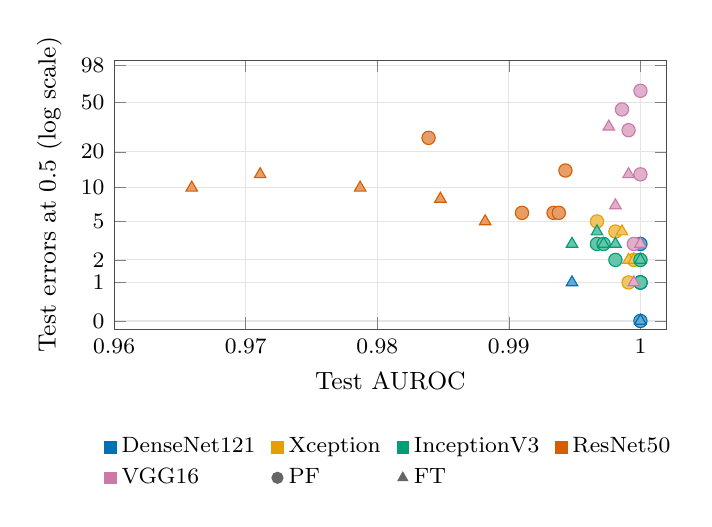
\begin{tikzpicture}
\begin{axis}[width=8.6cm, height=5.0cm, xmin=0.96, xmax=1.002, ymin=-0.15, ymax=4.6951,
  ytick={0.0000,0.6931,1.0986,1.7918,2.3979,3.0445,3.9318,4.5951}, yticklabels={0,1,2,5,10,20,50,98}, xlabel={Test AUROC}, ylabel={Test errors at 0.5 (log scale)},
  xticklabel style={/pgf/number format/fixed, /pgf/number format/precision=3},
  ticklabel style={font=\footnotesize}, label style={font=\small}, grid=major, grid style={black!10},
  axis line style={black!70}, legend cell align=left,
  legend style={font=\footnotesize, draw=none, legend columns=4, at={(0.5,-0.36)}, anchor=north,
  /tikz/every even column/.append style={column sep=4pt}}]

\addplot[only marks, mark=*, mark size=2.4pt, c1, mark options={fill=c1!60, draw=c1}, forget plot] coordinates {(1.0000,0.6931) (1.0000,0.6931) (1.0000,1.3863) (1.0000,0.6931) (1.0000,0.0000)};
\addplot[only marks, mark=triangle*, mark size=2.4pt, c1, mark options={fill=c1!60, draw=c1}, forget plot] coordinates {(1.0000,0.0000) (1.0000,0.0000) (1.0000,1.3863) (0.9948,0.6931) (1.0000,0.6931)};
\addplot[only marks, mark=*, mark size=2.4pt, c2, mark options={fill=c2!60, draw=c2}, forget plot] coordinates {(0.9967,1.7918) (0.9991,0.6931) (0.9995,1.0986) (1.0000,1.0986) (0.9981,1.6094)};
\addplot[only marks, mark=triangle*, mark size=2.4pt, c2, mark options={fill=c2!60, draw=c2}, forget plot] coordinates {(0.9986,1.6094) (0.9995,1.0986) (0.9991,1.0986) (0.9967,1.3863) (0.9995,1.0986)};
\addplot[only marks, mark=*, mark size=2.4pt, c3, mark options={fill=c3!60, draw=c3}, forget plot] coordinates {(0.9981,1.0986) (0.9967,1.3863) (1.0000,0.6931) (0.9972,1.3863) (1.0000,1.0986)};
\addplot[only marks, mark=triangle*, mark size=2.4pt, c3, mark options={fill=c3!60, draw=c3}, forget plot] coordinates {(0.9967,1.6094) (0.9948,1.3863) (0.9981,1.3863) (1.0000,1.0986) (0.9972,1.3863)};
\addplot[only marks, mark=*, mark size=2.4pt, c4, mark options={fill=c4!60, draw=c4}, forget plot] coordinates {(0.9934,1.9459) (0.9910,1.9459) (0.9938,1.9459) (0.9839,3.2958) (0.9943,2.7081)};
\addplot[only marks, mark=triangle*, mark size=2.4pt, c4, mark options={fill=c4!60, draw=c4}, forget plot] coordinates {(0.9848,2.1972) (0.9711,2.6391) (0.9659,2.3979) (0.9882,1.7918) (0.9787,2.3979)};
\addplot[only marks, mark=*, mark size=2.4pt, c5, mark options={fill=c5!60, draw=c5}, forget plot] coordinates {(1.0000,2.6391) (1.0000,4.1431) (0.9995,1.3863) (0.9991,3.4340) (0.9986,3.8067)};
\addplot[only marks, mark=triangle*, mark size=2.4pt, c5, mark options={fill=c5!60, draw=c5}, forget plot] coordinates {(0.9991,2.6391) (0.9981,2.0794) (1.0000,1.3863) (0.9976,3.4965) (0.9995,0.6931)};
\addlegendimage{only marks, mark=square*, c1}\addlegendentry{DenseNet121}
\addlegendimage{only marks, mark=square*, c2}\addlegendentry{Xception}
\addlegendimage{only marks, mark=square*, c3}\addlegendentry{InceptionV3}
\addlegendimage{only marks, mark=square*, c4}\addlegendentry{ResNet50}
\addlegendimage{only marks, mark=square*, c5}\addlegendentry{VGG16}
\addlegendimage{only marks, mark=*, black!60}\addlegendentry{PF}
\addlegendimage{only marks, mark=triangle*, black!60}\addlegendentry{FT}
\end{axis}
\end{tikzpicture}
\end{document}
